\documentclass[11pt,a4paper,titlepage, ngerman]{article}

\usepackage[utf8]{inputenc}	
\usepackage[T1]{fontenc}	
\usepackage{ngerman}			
\usepackage{lmodern}			
\usepackage{graphicx}			
\usepackage{url}				
\usepackage{siunitx}
\usepackage{amsmath}			
\usepackage{subcaption}
\usepackage{wrapfig}
\usepackage{biblatex}

\newcommand{\refeq}[1]{Gl. (\ref{eq:#1})}
\newcommand{\refabb}[1]{Abb. \ref{abb:#1}}
\newcommand{\reffig}[1]{Fig. \ref{fig:#1}}
\newcommand{\reftab}[1]{Tab. \ref{tab:#1}}

\begin{document}

	\begin{titlepage}
		
		\centering
		{\scshape\LARGE Versuchsbericht zu \par}
		\vspace{1cm}
		{\scshape\huge M1 -- Drehpendel nach Pohl\par}
		\vspace{2.5cm}
		{\LARGE Gruppe 10 Mi\par}
		\vspace{0.5cm}
		{\large Alex Oster (E-Mail: a\_oste16@uni--muenster.de) \par}
		{\large Jonathan Sigrist (E-Mail: j\_sigr01@uni--muenster.de) \par}
		\vfill
		durchgeführt am 15.11.2017\par
		betreut von\par
		{\large Johann Preuß}		
		\vfill	
		{\large \today\par}
		
	\end{titlepage}
		
	\tableofcontents
		
	\newpage
	
	\section{Kurzfassung}
		
		In diesem Bericht beschäftigen wir uns mit der Betrachtung verschiedener Typen von Schwingungen. Um diese genauer zu untersuchen verwenden wir das \glqq Drehpendel nach Pohl\grqq {}. Dieser Aufbau ermöglicht es uns freie, gedämpfte und erzwungene Schwingungen zu erzeugen. Auch das Einbringen einer Nichtlinearität ist hierbei möglich.	
			
		Zu jedem dieser Schwingungstypen führen wir mit Hilfe des Pendels Versuche durch. Anhand der Messergebnisse bestimmen wir dann die Eigenfrequenzen für die harmonischen Schwingungen bei unterschiedlichen Dämpfungen sowie die Resonanzfrequenzen und Phasenbeziehungen für erzwungene Schwingungen und wie diese sich mit Einführung einer Nichtlinearität verändern. 
		
		Zunächst gehen wir jedoch noch auf die Funktionsweise des Drehpendels, sowie die bei der Messung entstehenden Unsicherheiten ein.  		 
		
	\section{Pohl'sches Rad}
		
		Das Drehpendel nach Pohl oder auch Pohl'sches Rad ist wie in Abbildung \ref{abb:Drehpendel} zu sehen aufgebaut.
		Die zu sehende Scheibe ist mit einer Spiralfeder verbunden und erfährt bei Auslenkung die Rückstellkraft dieser. Dies führt zu einer Schwingung.
		Dabei lässt sich die Auslenkung an dem Maß außerhalb der Scheibe mit Hilfe des Pfeils, welcher an dieser angebracht ist, ablesen. 
		Zusätzlich ist an der Scheibe ein Faden angebracht, welcher mit einem Messgerät verbunden ist, um die Auslenkung zu bestimmen. Ein Computer, welcher an das Messgerät geschlossen ist, wertet die gemessenen Auslenkungen aus und trägt diese gegen die Zeit auf. 
		
		Die verschiedenen Schwingungstypen lassen sich mit dem Drehpendel wie folgt darstellen:
		\begin{description}
			\item[Freie Schwingungen:] 
				Diese lassen sich ohne äußeren Einfluss durch einfaches Auslenken des Pendels simulieren.
			\item[Gedämpfte Schwingungen:]
				 Durch Inbetriebnahme der Wirbelstrombremse, welche an dem unteren Teil der Scheibe angebracht ist, können gedämpfte Schwingungen erzeugt werden (vgl. \refabb{Drehpendel}). Die Stärke der Dämpfung lässt sich dabei durch Ändern der anliegenden Stromstärke anpassen. 
			\item[Erzwungene Schwingungen]
				Über einen Motor, welcher über einen Exzenter an den Aufbau verbunden ist, kann das Schwingen des Pendels erzwungen werden. 
			\item[Nichtlineare Schwingungen]
				Nichtlinearitäten treten bei der Schwingung auf, wenn man an die Scheibe des Drehpendels ein Gewicht anhängt.
		\end{description}
		\begin{figure}[ht]
			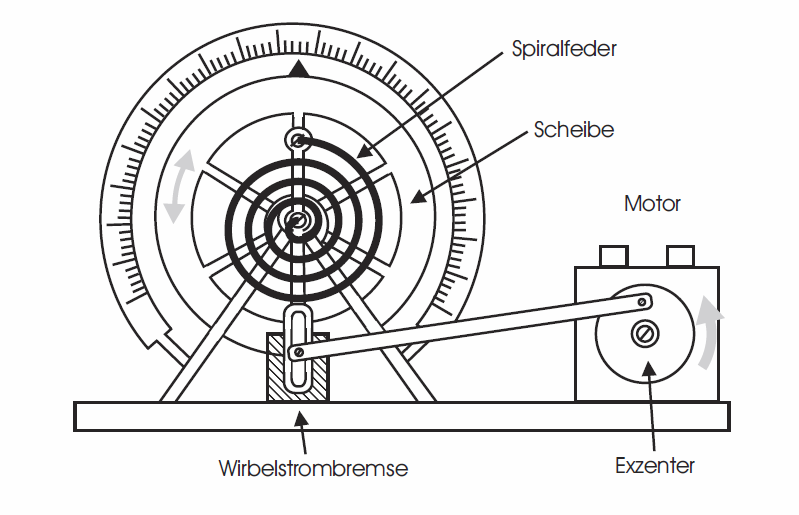
\includegraphics[width=\textwidth]{Drehpendel.png}
			\caption{Drehpendel nach Pohl}
			\label{abb:Drehpendel}
		\end{figure}
		
	\section{Messunsicherheiten der folgenden Versuche}
		
		Sehr unsicher.
		%TODO
		% Computermessung (?)
		% Stoppuhr (Digital + Reaktionszeit)
		% Multimeter (Digitalanzeige + 0,5% des Wertes)
		% Stromquelle (Digitalanzeige)
		% Auslenkungsbestimmung (Fehlertoleranzbereich von +- 1mm) ?
	
	\section{Versuch zu freien Schwingungen}
		
		Bei dem ersten Versuch befassen wir uns mit freien Schwingungen, welche wir mit dem Drehpendel nach Pol imitieren. Für diese Schwingung bestimmen wir anhand unserer Messungen die Eigenfrequenz bzw. die des Pendels.
		
		\subsection*{Methoden}
			
			Zur Bestimmung der Eigenfrequenz betrachten wir zunächst harmonische Schwingungen.					
			Für einen Drehschwinger mit Trägheitsmoment der Kreisscheibe $J$, rücktreibendem Drehmoment $-D\varphi$ (wobei $D$ Federkonstante) und bremsendem Drehmoment $-r\dot{\varphi}$, welches proportional zur Winkelgeschwindigkeit $\omega$ ist, lautet die Bewegungsgleichung der harmonischen Schwingung:
			\begin{align} %TODO schöner machen
				J\ddot{\varphi}+r\dot{\varphi}+D\varphi=0 \\
				\text{und in der Normalform: } \ddot{\varphi}+2\rho\dot{\varphi}+\omega_0^2\varphi=0 \label{eq:HarmonischeSchwingung}\\
				\text{wobei: } \omega_0^2 = \frac{D}{J} \text{und } 2\rho = \frac{r}{J}
			\end{align} 
			Da wir bei der freien Schwingung jedoch keine Dämpfung vorliegen haben, ist $2\rho = 0$ und $\omega_0$ somit unsere Eigenfrequenz.
			
			Wir bestimmen die Eigenfrequenz des Pendel in diesem Versuch einmal über die Messung, die der Computer durchführt und einmal indem wir die Zeit, welche das Pendel für zehn Schwingungen braucht, mit einer Stoppuhr messen.
		
		\subsection*{Messung}
			
			- - -
			%TODO
			% Messung
			
		\subsection*{Schlussfolgerung}
			
			- - -
			%TODO
			% Schlussfolgerung
				
	\section{Versuch zu gedämpften Schwingungen}
		
		In diesem Versuch betrachten wir gedämpfte Schwingungen, welche ebenfalls harmonisch sind.
		Zum Dämpfen des Pendels verwenden wir die Wirbelstrombremse, wie oben beschrieben. 
				
		\subsection*{Methoden}
			
			Betrachten wir nun erneut \refeq{HarmonischeSchwingung}, wobei dieses mal $2\rho \neq 0$ ist, so
			erhalten wir mit dem Ansatz $\varphi (t)=C\cdot e^{\omega t}$ die Lösung: 
			\begin{equation}
				\omega_{1,2}= -\rho \pm \sqrt{\rho^2-\omega_0^2}
			\end{equation}
			An dieser Stelle müssen wir differenzieren, in welchem Verhältnis $\rho$ und $\omega_0$ stehen.
			%TODO 3Fälle kurz beschreiben
						
			Hier und in den folgenden Versuchen betrachten wir nur noch die von dem Computer aufgenommenen Messergebnisse. Wir messen auch hier die Zeit, dieses mal jedoch bis das Pendel komplett aufhört zu schwingen und führen die Messung für verschiedene Dämpfungen durch. Um die Stärke der Dämpfung einzustellen betrachten wir verschiedene Eingabestromstärken für die Wirbelstrombremse.
		
		\subsection*{Messung}
		
			- - -
			%TODO
			% Messung
			
		\subsection*{Schlussfolgerung}
			
			- - -
			%TODO
			% Schlussfolgerung
			
	\section{Versuch zu erzwungenen Schwingungen}
	
		Nun betrachten wir erzwungene Schwingungen %TODO
			
		\subsection*{Methoden}
			
			\subsubsection*{Erzwungene Schwingungen}
			
				%TODO
				% Beschreibung erzwungene Schwingung
				
			\subsubsection*{Bestimmung der Resonanzfrequenz}
			
				%TODO
				% Bestimmung der Resonanzfrequenz bei erzwungener Schwingung
				% Frequenz der Anregung (Kalibrierkurve)
					% Frequenz über Ausgangsspannung (mit Multimeter gemessen)
				% Resonanzfrequenzbestimmung bei 3 Dämpfungen mit min. 20 Messpunkten
				% Darstellen dieser Resonanzkurven
				
			\subsubsection*{Phasenverschiebung}
			
				%TODO
				% Betrachtung der Phasenverschiebung zwischen Anreger und Pendel
					% bei schwacher/starker Dämpfung und niedriger/hoher Frequenz
					% Auf Fadenpendel übertragen
		
		\subsection*{Messung}
		
			%TODO
			% Messung
			
		\subsection*{Schlussfolgerung}
		
			%TODO
			% Schlussfolgerung
			
	\section{Versuch zu nichtlinearen Schwingungen}
	
		Der letzte Versuch behandelt nichtlineare Schwingungen. %TODO
		
		\subsection*{Methoden}
			
			\subsubsection*{nichtlineare Schwingungen}
			
				%TODO
				% Beschreibung nichtlineare Schwingung
			
			\subsubsection*{Resonanzbetrachtung}
			
				%TODO
				% Einbringen einer Nichtlinearität und Betrachtung der Resonanz
		
		\subsection*{Messung}
			
			%TODO
			% Messung
			
		\subsection*{Schlussfolgerung}
			
			%TODO
			% Schlussfolgerung

	\newpage			
	\section*{Literatur}
		\begin{description}
			\item[\refabb{Drehpendel}] Das hier verwendete Bild stammt aus \glqq Drehpendel\_Pohl\_Einführung.pdf\grqq
		\end{description}
\end{document} 